% Supplemental Material for "Coordination three heals, coordination four is hard".
% Compile:  latexmk -pdf supplementary.tex   (shares refs.bib and figs/ with main.tex)
% Items marked \verify{...} must be checked against the journal version of Ref. [Johnson2025]
% (Algorithmica 87, 429-464 (2025)) or the cited source before submission.
% Referee check of this note: ../reviews/supp_s1_review.md
\documentclass[aps,pre,onecolumn,superscriptaddress,nofootinbib]{revtex4-2}
\usepackage{amsmath,amssymb,amsthm}
\usepackage{graphicx}
\usepackage{xcolor}
\usepackage{hyperref}

\newtheorem{theorem}{Theorem}
\renewcommand{\thetheorem}{S\arabic{theorem}}
\newtheorem{lemma}[theorem]{Lemma}
\newtheorem{proposition}[theorem]{Proposition}
\theoremstyle{remark}
\newtheorem{remark}[theorem]{Remark}
\renewcommand{\thetable}{S\arabic{table}}
\renewcommand{\thefigure}{S\arabic{figure}}
\renewcommand{\theequation}{S\arabic{equation}}

\newcommand{\fr}{\operatorname{fr}}
\newcommand{\ioct}{\operatorname{ioct}}
\newcommand{\verify}[1]{\textcolor{red}{[VERIFY: #1]}}

\begin{document}

\title{Supplemental Material for ``Coordination three heals, coordination four is hard:
the antiferromagnetic Potts model with a costly third state''}
\author{[TODO authors]}
\affiliation{[TODO affiliation]}
\date{\today}
\maketitle

\section*{Note A. Independent odd cycle transversal on planar subcubic graphs}

The healing theorem of the main text (restated as Theorem~\ref{thm:S-heal}) implies that
independent odd cycle transversal is solvable in polynomial time on planar graphs of maximum
degree three. Reference~\cite{Johnson2025} states that this problem is NP-complete on that class.
This note explains the difference in detail. We separate what the proof in Ref.~\cite{Johnson2025}
establishes, what our theorem implies, and the one step, the planarity of the constructed graphs,
where our analysis differs from that proof. All numbers are reproducible with the scripts listed
in Sec.~A.7.

\subsection*{A.1 The two statements}

An \emph{independent odd cycle transversal} (IOCT) of a graph $G$ is an independent vertex set
$S$ such that $G-S$ is bipartite; $\ioct(G)$ is its minimum size ($\infty$ if none exists).
$\fr(G)=|E|-\mathrm{maxcut}(G)$ is the minimum number of monochromatic edges of a 2-colouring.
For graphs of maximum degree at most three, $\ioct(G)\ge\fr(G)$: re-inserting a vertex of degree at
most three on the side where it has fewer neighbours creates at most one monochromatic edge. (For
larger degree the inequality can fail; the wheel $W_4$ has $\ioct=1<2=\fr$.)

\begin{theorem}[main text, healing theorem]\label{thm:S-heal}
Every graph of maximum degree at most three without a $K_4$ component satisfies $\ioct(G)=\fr(G)$.
\end{theorem}

In Ref.~\cite{Johnson2025} the problem is defined as deciding whether a graph has an independent
odd cycle transversal of size at most $k$ for a given integer $k$ (p.~445). Theorem~11 there reads:
``List Colouring, Odd Cycle Transversal and Independent Odd Cycle Transversal are C123-problems''
(p.~445). Condition C2 is that the problem is ``computationally hard for the class of subcubic
graphs'' (p.~434), without planarity. \emph{Theorem~11 itself is therefore consistent with
Theorem~\ref{thm:S-heal}}; see Sec.~A.2. The statement that differs is an additional one, made
in the text around Theorem~11: ``Our proof shows in particular that all three problems are in
fact NP-complete for planar subcubic graphs'' (p.~445), repeated on p.~438 (``we prove, as new
results, that List Colouring, Odd Cycle Transversal, Independent Odd Cycle Transversal, and
C$_5$-Colouring are NP-complete for planar subcubic graphs''), and reflected in the entries of
Table~1 for planar and subcubic planar graphs.

On planar graphs $\fr(G)$ is computable in polynomial time (maximum cut of a planar graph via a
minimum $T$-join in the dual~\cite{Hadlock1975,Barahona1982}). By Theorem~\ref{thm:S-heal} the
question ``$\ioct(G)\le k$?'' on a planar graph of maximum degree three has the answer yes if and
only if $G$ has no $K_4$ component and $\fr(G)\le k$. (A $K_4$ component admits no IOCT; $\ioct$
and $\fr$ are additive over components; vertices of degree below three are covered by the
theorem.) The question is therefore decidable in polynomial time. If the problem were also
NP-complete on this class, P would equal NP.

The same construction is used in Ref.~\cite{Johnson2025} for (not necessarily independent) Odd
Cycle Transversal. For that problem, polynomial-time solvability on planar subcubic graphs already
follows from Theorem~1 of Choi, Nakajima and Rim~\cite{Choi1989}, which states that for graphs of
maximum degree three the minimum odd cycle transversal (vertex bipartization) has the same size as
the minimum edge bipartization, $\fr(G)$, combined with planar maximum cut. Theorem~\ref{thm:S-heal}
strengthens that result by requiring the transversal to be independent. We make no statement
about the other problems treated with the same construction.

\subsection*{A.2 Points of agreement}

\begin{enumerate}
\item \emph{Theorem~11 as stated.} C2 asks for hardness on subcubic graphs, and C3 for hardness
under edge subdivision of subcubic graphs; neither requires planarity (p.~434). The arguments
below do not affect either.
\item \emph{The reduction's equivalence.} The proof in Ref.~\cite{Johnson2025} builds, from a
3-SAT formula $\varphi$ with $m$ clauses, a subcubic graph $G_\varphi$ with $2m$ vertex-disjoint
triangles (two in each clause gadget), such that $G_\varphi$ has an IOCT of size $2m$ if and only
if $\varphi$ is satisfiable (pp.~445--446). We
have found no problem with this equivalence and checked it by exact integer programming on 80
random formulas (70 satisfiable, 10 unsatisfiable) and on every instance of Table~\ref{tab:S-inst},
with agreement in all cases.
\item \emph{NP-completeness on general subcubic graphs.} The equivalence gives NP-completeness of
IOCT on graphs of maximum degree three that need not be planar. This is consistent with
Theorem~\ref{thm:S-heal}, which yields the same conclusion from the NP-hardness of maximum cut on
cubic graphs~\cite{Yannakakis1978} \verify{cubic max-cut NP-hardness reference}.
\item \emph{Other results.} This note concerns no other result of Ref.~\cite{Johnson2025}.
\end{enumerate}
The difference concerns only whether $G_\varphi$ is planar for every instance $\varphi$ of the
planar 3-SAT variant used in Ref.~\cite{Johnson2025}. Consequences drawn in that paper from
hardness on planar subcubic graphs (for instance through its Theorem~2) would, for Odd Cycle
Transversal and Independent Odd Cycle Transversal, need to be revisited; we do not pursue this.

\subsection*{A.3 The construction and the features used here}

The instances are those of Planar 3-Satisfiability ``when each literal appears in at most two
clauses'', with two-literal or three-literal clauses, where planar means that ``the bipartite
incidence graph of clauses with variables is planar'' (p.~445--446, citing Theorem~2 of
Ref.~\cite{DarmannDockerDorn2018}). From $\varphi$ the graph $G_\varphi$ is built as follows
(p.~445--446): literal vertices $x_i$, $\bar x_i$ with the edge $x_i\bar x_i$; a path $P$ of $2m$
vertices; for each clause a copy of the gadget of Fig.~3 there, whose input vertices
$c_{j1},c_{j2},c_{j3}$ are identified with the literal vertices of the clause; an edge from the
output $c_j$ to the $j$th odd vertex of $P$; and an edge from any unused input $c_{j3}$ to the
$j$th even vertex of $P$. Our implementation \texttt{verify\_delta3\_reduction.build} follows this
description; its clause gadget (vertices $a,b,d,e,f,c$ with edges $ab$, $ad$, $bd$, $de$, $ef$, $ec$,
$fc$ and inputs attached to $a$, $b$, $f$) agrees with Fig.~3 of Ref.~\cite{Johnson2025}. We use
only the following features:
\begin{enumerate}
\item[(F0)] the literal vertices, the vertices $u_j$ below, the gadgets $Q_j$ and the path $P$ are
pairwise disjoint vertex sets;
\item[(F1)] each variable $x_i$ is represented by two literal vertices $x_i$, $\bar x_i$ joined by
an edge;
\item[(F2)] each clause $C_j$ is represented by a connected gadget $Q_j$ (two triangles and
connecting edges) that is adjacent to the literal vertex of every literal of $C_j$; for a
two-literal clause the third input of $Q_j$ is a private vertex $u_j$;
\item[(F3)] a path $P$, which carries the truth values, is adjacent to every gadget $Q_j$.
\end{enumerate}
Planarity of $G_\varphi$ is argued in Ref.~\cite{Johnson2025} as follows (p.~446): ``In Planar
3-Satisfiability, the bipartite incidence graph of clauses with variables is planar. We build $G$
so as to be planar in the following way. Uppermost we place the literals assigned to the inputs
of the clause gadgets in just the manner prescribed in the bipartite incidence graph. Lowermost,
we place the path of length $2m$ that will be joined on the odd vertices to the output nodes of the
clause gadgets.'' The step from planarity of the incidence graph to planarity of $G_\varphi$ is the
one examined below.

\subsection*{A.4 A minor of $G_\varphi$}

Let $I(\varphi)$ be the variable--clause incidence graph of $\varphi$ (one vertex per variable and
one per clause; an edge when the variable occurs in the clause, with either sign), and let
$H(\varphi)$ be $I(\varphi)$ together with one new vertex $p$ adjacent to every clause vertex.

\begin{lemma}\label{lem:S-minor}
Under (F0)--(F3), $H(\varphi)$ is a minor of $G_\varphi$, for every order of the clauses along $P$
and every assignment of literals to gadget inputs.
\end{lemma}

\begin{proof}
Delete the vertices $u_j$. Contract the path $P$ to one vertex $p$, each gadget $Q_j$ to one vertex
$C_j$, and each edge $x_i\bar x_i$ to one vertex $x_i$; each contracted set is connected (F1--F3)
and the sets are disjoint (F0). By (F2) the vertex $C_j$ is adjacent to every variable occurring in
$C_j$, and by (F3) to $p$. Removing parallel edges and any further edges leaves $H(\varphi)$. No
property of the orders is used.
\end{proof}

Since every minor of a planar graph is planar:

\begin{proposition}\label{prop:S-criterion}
If $H(\varphi)$ is non-planar, then $G_\varphi$ is non-planar for every clause order and every
literal order.
\end{proposition}

Planarity of $I(\varphi)$ does not imply planarity of $H(\varphi)$: $H(\varphi)$ is planar exactly
when $I(\varphi)$ has a planar drawing with all clause vertices on one face. Features (F1) and (F3)
are both needed for the minor; without the edges $x_i\bar x_i$, for example, the corresponding
graph is planar for all instances below.

\subsection*{A.5 Explicit instances}

The smallest instance is
\begin{equation}
\varphi^* = (x\vee y)\wedge(\bar x\vee y)\wedge(x\vee\bar y).
\end{equation}
Every literal occurs at most twice, every variable exactly three times with both signs, and
$I(\varphi^*)=K_{2,3}$ is planar. But $H(\varphi^*)=K_{3,3}$, with parts $\{C_1,C_2,C_3\}$ and
$\{p,x,y\}$, because each clause contains both variables and is adjacent to $p$
(Fig.~\ref{fig:S-minor}). By Proposition~\ref{prop:S-criterion}, $G_{\varphi^*}$ (31 vertices, 43
edges) is non-planar for every choice of orders. As an independent check, a planarity test on
$G_{\varphi^*}$ itself returns a Kuratowski subgraph, a subdivision of $K_{3,3}$, drawn in red in
Fig.~\ref{fig:S-minor}(a).

\begin{figure}[h]
\centering
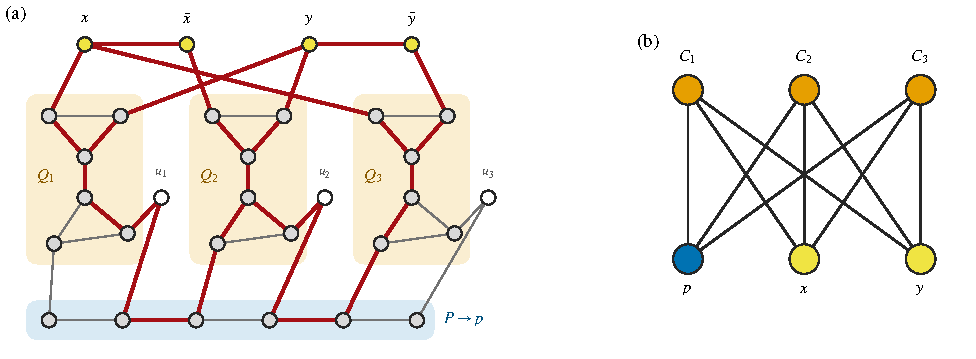
\includegraphics[width=\textwidth]{figs/fig_supp_minor.pdf}
\caption{(a) The reduction graph $G_{\varphi^*}$ for $\varphi^*=(x\vee y)(\bar x\vee y)(x\vee\bar y)$,
as implemented in \texttt{verify\_delta3\_reduction.build}. Top: literal vertices; shaded: the clause
gadgets $Q_1,Q_2,Q_3$ and the path $P$; white: the unused third inputs $u_j$. Red: one Kuratowski
subgraph (subdivided $K_{3,3}$) returned by a planarity test. (b) Contracting each shaded set and
each literal edge and deleting the $u_j$ gives $H(\varphi^*)=K_{3,3}$ (Lemma~\ref{lem:S-minor}).}
\label{fig:S-minor}
\end{figure}

Planar 3-SAT is used in several variants: ``planar'' may refer to $I(\varphi)$ alone or to $I(\varphi)$
plus a cycle through the variables (Lichtenstein's original formulation~\cite{Lichtenstein1982}),
and variants restrict clause sizes and the number of occurrences. Table~\ref{tab:S-inst} lists
instances covering these conditions, including unsatisfiable ones. Every instance in the table
satisfies the conditions used in Ref.~\cite{Johnson2025}: two- or three-literal clauses, each
literal in at most two clauses, and planar incidence graph. Formulas with
exactly three literals per clause and at most three occurrences per variable are always
satisfiable~\cite{Tovey1984}; for that reason the instance $\varphi_{\mathrm B}$ uses four
occurrences per variable.

\begin{table}[h]
\caption{Instances $\varphi$ with planar incidence graph $I(\varphi)$, non-planar $H(\varphi)$ and
hence non-planar $G_\varphi$. Literals are written $\pm i$ for $x_i$, $\bar x_i$. ``lit'': maximum
occurrences of a literal; ``var'': occurrences of a variable; ``var.\ cycle'': a variable order for
which $I(\varphi)$ plus the cycle through the variables in that order is planar (Lichtenstein's
condition); $|V|,|E|$: size of $G_\varphi$. The reduction equivalence was confirmed by exact
optimisation for each instance.}
\label{tab:S-inst}
\begin{ruledtabular}
\begin{tabular}{llccccccc}
& $\varphi$ & sizes & lit & var & var.\ cycle & sat. & $H(\varphi)$ & $|V|,|E|$\\
\hline
$\varphi^*$ & $(1,2)(-1,2)(1,-2)$ & 2 & 2 & 3 & (2 variables) & yes & $K_{3,3}$ & 31, 43\\
$\varphi_{23}$ & $(2,-1,-3)(1,2)(-3,1)(-2,3)$ & 2, 3 & 2 & 3 & 1,2,3 & yes & non-planar & 41, 57\\
$\varphi_{\mathrm B}$ & $(-5,-4,2)(-6,-3,4)(3,5,1)(-6,3,1)$ & 3 & 2 & 4 & 1,2,4,5,3,6 & yes & non-planar & 76, 109\\
 & $\;\;(4,6,-2)(-1,-5,2)(5,-4,-3)(-2,-1,6)$ & & & & & & & \\
$\varphi_{\mathrm U}$ & $(-4,-2)(4,5)(3,1)(-2,4,-5)(-5,-3)(2,-1)(1,-3)$ & 2, 3 & 2 & 3 & 1,2,3,4,5 & no & non-planar & 72, 101\\
$\varphi_{2\mathrm U}$ & $(1,-3)(4,-2)(-2,1)(-3,4)(-4,-1)(3,2)$ & 2 & 2 & 3 & 1,2,3,4 & no & non-planar & 62, 87\\
$\varphi_0$ & $(5,2)(4,-5)(1,-6)(6,3)(3,-4)(6,4,-2)$ & 2, 3 & 2 & $\le4$ & 1,2,4,3,5,6 & yes & non-planar & 92, 130\\
 & $\;\;(-2,1)(-1,5)(-6,-1)$ & & & & & & & \\
\end{tabular}
\end{ruledtabular}
\end{table}

For $\varphi_{23}$ the $K_{3,3}$ minor can be read off by hand: parts $\{C_1,C_3,C_4\}$ and
$\{p,x_1,x_3\}$, where the edge $C_4x_1$ is realised by the path $C_4\,x_2\,C_2\,x_1$ in
$H(\varphi_{23})$.

\emph{Random instances.} Among 131 random formulas with clause sizes 2--3, every literal at most
twice, every variable at most three times, 5--14 variables and planar $I(\varphi)$, 130 have
non-planar $H(\varphi)$ and non-planar $G_\varphi$. There was no case with non-planar $H(\varphi)$
and planar $G_\varphi$, as Lemma~\ref{lem:S-minor} requires.

\subsection*{A.6 A structural reason}

The instances show that planarity of $G_\varphi$ does not follow from planarity of $I(\varphi)$.
The following argument, which does not use Theorem~\ref{thm:S-heal}, indicates that it cannot hold
on hard formulas for a construction with features (F0)--(F3).

Suppose $G_\varphi$ is planar. Then $H(\varphi)$ is planar (Lemma~\ref{lem:S-minor}). In a planar
drawing of $H(\varphi)$, draw a small circle around $p$ that meets each edge at $p$ once, delete $p$
and the parts of these edges inside the circle, and contract the remaining parts of these edges.
The result is a planar drawing of $I(\varphi)$ plus a cycle through all clause vertices, with all
variable vertices on one side of the cycle. Satisfiability of such (``co-nested'') formulas is
decidable in polynomial time~\cite{KratochvilKrivanek1993}; see also Ref.~\cite{Pilz2019}, Sec.~1
\verify{confirm the definition of co-nested formulas and the polynomial-time result in
Kratochv\'il--K\v{r}iv\'anek 1993 and in Pilz 2019, Sec.~1}. Hence, unless P${}={}$NP, a reduction
whose graphs have features (F0)--(F3) produces planar graphs only on a class of formulas on which
satisfiability is not NP-hard.

\subsection*{A.7 Summary and reproducibility}

\begin{enumerate}
\item We have found no problem with the reduction equivalence of Ref.~\cite{Johnson2025}, and
NP-completeness of IOCT on general subcubic graphs is consistent with Theorem~\ref{thm:S-heal}.
\item In our analysis, planarity of $G_\varphi$ does not follow from planarity of the incidence
graph: it fails for the instances of Table~\ref{tab:S-inst} under every clause and literal order
(Lemma~\ref{lem:S-minor}), and for constructions with features (F0)--(F3) it can hold only on
formulas whose satisfiability is decidable in polynomial time (Sec.~A.6).
\item Theorem~\ref{thm:S-heal} gives a polynomial algorithm for IOCT on planar subcubic graphs. Its
proof is independent of the above; it is supported by computational checks: exhaustive to 12
vertices, and exact optimisation on 251 graphs of 14--60 vertices, including reduction graphs
$G_\varphi$ (main text, Appendix), and on 1,386 further graphs of 16--100 vertices
(\texttt{reviews/c5\_review2\_milp.py}).
\end{enumerate}

Scripts in the \texttt{d3\_complexity/} folder of the code repository \verify{repository URL or
Zenodo DOI}:
\begin{itemize}
\item \texttt{python3 supp\_planarity.py 300 1}: Table~\ref{tab:S-inst}, the random-instance
statistics and Kuratowski subgraphs; output \texttt{supp\_runs/planarity\_evidence.json};
\item \texttt{python3 verify\_delta3\_reduction.py}: the reduction equivalence on 80 formulas;
\item \texttt{cd paper \&\& python3 make\_supp\_figs.py}: Fig.~\ref{fig:S-minor}.
\end{itemize}

\bibliography{refs}

\end{document}
